\documentclass[a4paper]{article}
\usepackage[utf8]{inputenc}
\usepackage[frenchb]{babel}
\usepackage{tikz}
\usepackage{ifpdf}
\usepackage{graphicx}
\usepackage{hyperref}

\title{Octochat \\ \textit{Le chat décentralisé}}
\author{Alexis \textsc{Giraudet} \and Benjamin \textsc{Sientzoff}}
\date{\today}
\ifpdf
\hypersetup{
    pdfauthor={Alexis Giraudet, Benjamin Sientzoff},
    pdftitle={Octochat - Discuter sur le réseau local sans serveur},
}
\fi
\begin{document}
	% page de garde avec sommaire
	\maketitle
	\vspace{9cm}
	\tableofcontents
	\newpage % passer à la page suivante

	\section*{Introduction}
		\paragraph{}{
		Ce projet a été réalisé dans le cadre du cours \textit{Objet et développement d'applications}
		dans lequel M. \textsc{Richoux} nous a enseigné l'utilisation des \textit{Design Patterns}.
		L'ambition de ce projet ne s'arrête pas là, car nous souhaitons poursuite le développement de notre
		programme. Le sujet de notre projet est la création d'un client de chat qui n'utilise pas de serveur
		principal comme c'est le cas pour ce genre d'application réseau. Le fonctionnement est détaillé plus loin.
		}
		\paragraph{}{
		Octochat, notre programme, est donc un client de chat qui n'a pas besoin de serveur pour fonctionner.
		Lancer le programme, choisissez un nom d'utilisateur est c'est parti. Cependant, la mise en place d'une telle
		application n'est pas aisée. Ce rapport retrace la conception d'Octochat jusqu'au 26 novembre 2014. Il met en évidence les points qui ont posés problèmes et les différents \textit{patterns} utilisés.
		}

	\newpage

	\section{Utilisation et fonctionnement global}

		\paragraph{Boost}{
		Pour des questions de dépendances et pour faciliter le développement du programme, notamment pour ce qui est du réseau,
		nous avons choisi d'utiliser la librairie \textit{Boost}.
		L’utilisation de cette librairie nous permet également d'utiliser le système de compilation associé.
		}

		\subsection{Compilation du programme}
			\paragraph{Compilation}{
			Notre programme utilise deux bibliothèques à savoir la librairie standard du langage ( \textit{STL} et \textit{Boost}, plus précisément:
			\begin{itemize}
				\item[Boost.Build] le système de compilation (équivalant de \textit{make} et des \textit{Makefile} mais plus portable)
				\item[Boost.Thread] pour les \textit{thread]} et les \textit{mutex}
				\item[Boost.Log] pour les \textit{logs}
				\item[Boost.Asio] pour les entrées/sorties asynchrones sur le réseau
				\item[Boost.Serialization] pour sérialiser les données envoyées sur le réseau
				\item[Boost.System] pour les \textit{Smart Pointers} et le \textit{Lexical Cast}
				\item[Boost.Uuid] pour la sérialisation
			\end{itemize}
			}
			\paragraph{}{
			Pour compiler notre programme nous avons donc besoin d’un compilateur (incluant la \textit{STL})
			et d’installer \textit{Boost}, c’est pourquoi nous avons réalisé un \textit{Makefile} qui s’occupe
			d’installer \textit{Boost} localement et de compiler le programme automatiquement.
			Une fois la compilation terminée, les exécutables sont placés dans le dossier \textit{build}:
			\begin{itemize}
				\item[octowatch] écoute le réseau
				\item[octoglobalchat] propose de chatter avec toutes les paires connectées
				\item[octochat] permet de chatter avec des utilisateurs
			\end{itemize}

			}
			\paragraph{Remarque}{
				Il est possible d’installer \textit{Boost} avec un gestionnaire de paquets à condition d’avoir les privilèges suffisants.
			}


			\paragraph{}{
				Pour compiler le projet, on commence par cloner le dépôt, puis on lance la commande make à la racine du projet.
			}

			\begin{verbatim}
				$ git clone https://github.com/blasterbug/Octochat.git
				$ cd Octochat
				$ make
			\end{verbatim}

		\subsection{Utilisation}
			\paragraph{}{
			Si toutes les précédentes étapes se sont bien passées, vous êtes maintenant en mesure d'utiliser Octochat.
			Pour lancer l'application taper simplement \verb|./octochat|
			}

		\subsection{Sous le capot}
			\paragraph{}{
			Dès le début, nous avons décidé de diviser notre application en couches.
			Une première couche s'occupe de la gestion du réseau à proprement parler. Une seconde couche,
			qui pourrait être découper elle aussi en deux parties s'occupe des aspect applicatif du programme.
			}

			\paragraph{Couche Réseau}{
			Lors du développement de la couche réseau, nous avons cherché à découplé le plus possible les
			applications clientes de l’application réseau c’est pourquoi nous avons utilisé le \textit{pattern
			abstract factory}. \\
			En ce qui concerne la communication des données entre la couche réseau et les application clientes,
			l’utilisation du \textit{pattern observer} s’est révélé naturel.
			}

			\paragraph{Couche réseau}{
			La couche applicatif permet de définir un protocole sur lequel Octochat peut reposer permettant ainsi
			de gérer les utilisateurs d'un salon (une \textit{octoroom}), leur connexion et leur déconnexion au sein
			des salons.
			}
			
		\newpage

	\section{Patrons de conception}
	
		\section{abstract factory}
		
			\paragraph{}{
			Les pairs c’est à dire les instances de l’application réseau sont appelées octopeer, 
			une octopeer est identifiée de manière unique grâce à un UUID généré à sa création. \newline
			Une octopeer peut transmettre des données via une octoquery, une octoquery est composée
			 d’une string contenant les données (données sérialisées) et d’une octopeer correspondant à 
			 l’émetteur ou bien au destinataire suivant que l’on envoie ou bien que l’on reçoive cette octoquery.
			}
			
			\paragraph{}{
			Dans notre cas, nous avons voulu que “décentralisé” rime avec “autonomie”, c’est pourquoi nous 
			avons identifié deux services distincts capables de gérer les entrées/sorties des pairs.
			}
			\begin{itemize}
				\item Le premier service, est le service d’exploration qui consiste à identifier des pairs
				potentielles en vue de communiquer avec elles. Nous avons appelé ce service exploration\_server 
				(le mot serveur est un abus de langage mais dans ce cas le concept associé est plus intuitif). 
				Un service d’exploration très simple pourrait tout simplement consister à lire un fichier contenant
				des informations de connexions sur les pairs (ip/port, nom d'hôte…) ou bien de manière plus évoluée, 
				envoyer un broadcast sur le réseau local et observer les réponses puis tester ces pairs potentielles 
				grâce au second service.
				
				\item Le second service propose de tester si une pair se cache derrière les informations fournis 
				par l’explorateur, puis de transmettre des octoquery aux pairs vérifiées, il s’agit du communicator\_server.
			\end{itemize}
			
			\paragraph{}{
			L’avantage de cette approche est l’indépendance envers les protocoles de communications, en effet
			une octoquery peut très bien être encapsulée dans un paquet TCP ou bien être transférée via HTTP,
			 voire même fonctionner uniquement sur la boucle locale.
			}
			
			\begin{figure}[!h]
					\centering
					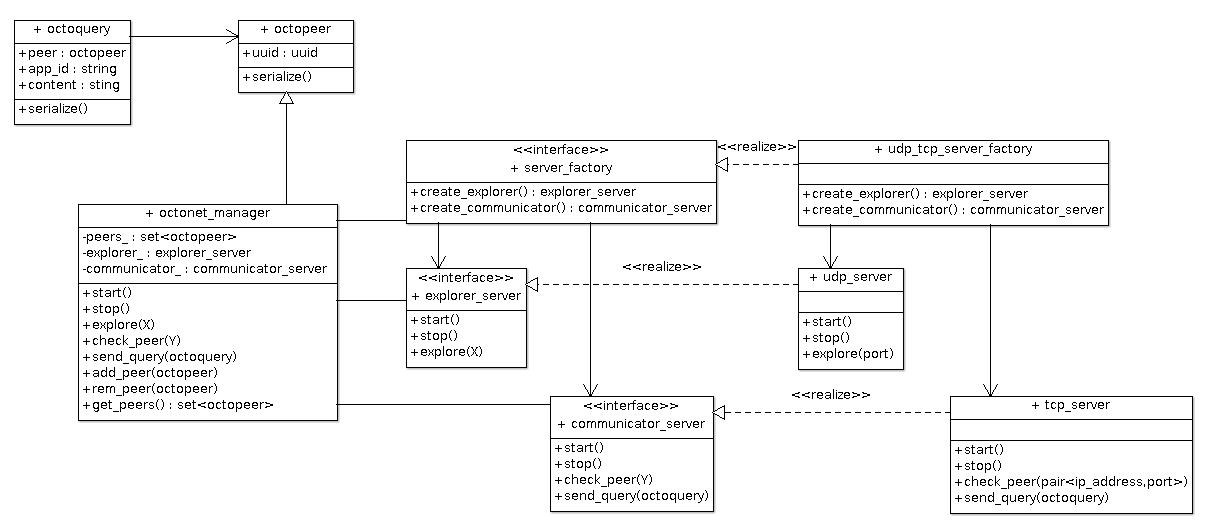
\includegraphics[scale=0.5]{UML/octonet_factory1.png}
					\caption{\label{factory_uml} Diagramme UML du \textit{pattern abstract factory}}
			\end{figure}
						
			
			\paragraph{}{
			Pour définir précisément ses services et orienter leur implémentation nous avons utilisé le
			\textit{pattern abstract factory}, comme on peut le voir à la figure \ref{factory_uml}.
			}
				\subparagraph{Remarque}{Sur le schéma UML à la figure \ref{factory_uml}, X et Y sont des types génériques.}
				
			\paragraph{}{
			Nous avons donc implémenté server\_factory avec le protocole UDP pour explorer le réseau et le
			protocole TCP pour la communication entre les pairs. \newline
			udp\_server: la fonction explore se charge d’envoyer un broadcast contenant les informations de
			connexion (à savoir l’adresse IP et le port du serveur de communication), la fonction run 
			se chargera donc de lancer le serveur qui réceptionnera ces informations pour les
			transmettre au communicator\_server.
			}
			
			\paragraph{}{
			tcp\_server: la fonction check\_peer se charge d’établir une connexion avec une potentielle octopeer
			(comme nous le vérons dans la partie sur le pattern observer, si la connexion réussie alors les
			octopeer\_observer seront notifiés), la fonction send\_query permet d’envoyer une octoquery et 
			run lance le serveur TCP qui recevra les octoquery (et notifiera les octoquery\_observer).
			}
			
			\paragraph{}{
			Nous avons donc implémenté server\_factory avec le protocole UDP/TCP, mais il est tout à fait 
			possible d’utiliser d’autres protocoles pouvant utiliser les noms de domaine par exemple.
			}

		\subsection{Observer}
		
			\paragraph{}{
			Ensuite pour interagir avec les applications nous avons naturellement utilisé le \textit{design pattern observer},
			visible à la figure \ref{observer_uml}.
			}

			\begin{figure}[!h]
				\centering
				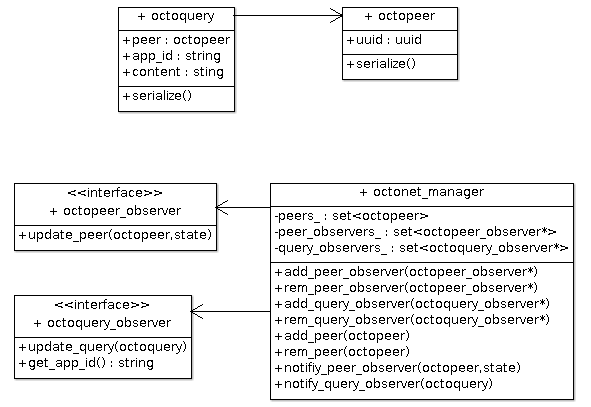
\includegraphics[scale=0.65]{UML/octonet_observer1.png}
				\caption{\label{observer_uml} Diagramme UML du \textit{pattern Observer}}
			\end{figure}
			
			\paragraph{}{
			En effet, les applications pourrons être notifiées de la connexion/déconnexion d’une
			\textit{octopeer} en implémentant l’interface \textit{octopeer\_observer}.
			}
			\paragraph{}{
			Ensuite les applications devront être notifiées de l’arrivée d’une nouvelle \textit{octoquery}. 
			Pour cela, nous avons rajouté un système de filtre très simple pour que les applications 
			puissent communiquer avec leurs homologues distant voir même avec d’autres applications. \newline
			Pour cela, nous avons ajouté un membre \textit{app\_id} aux \textit{octoquery} et les applications réalisant 
			l’interface octoquery\_observer retournent leur propre app\_id. Donc, lorsqu’une octoquery
			est reçue, seules les applications ayant le même \textit{app\_id} que l’\textit{octoquery} sont notifiées 
			(un \textit{octoquery\_observer} retournant un \textit{app\_id} vide sera toujours notifié).
			}

			\paragraph{}{
			Ce système de notifications permet donc à divers applications d’interagir ensemble, prenons par 
			exemple une application de partage de fichiers et une application de chat: on pourrait très bien 
			imaginer la possibilité d’utiliser ces deux applications de manière complémentaire, c’est à dire 
			pouvoir partager des fichiers dans le chat.
			}
			
			\paragraph{}{
			La classe \textit{octonet\_manager} est donc à la fois la classe cliente du pattern abstract \textit{factory} 
			mais aussi la classe observable du \textit{pattern observer}, nous avons donc rajouté la façade 
			\textit{octonet} pour masquer certaines fonctionnalités aux applications (notamment les fonctions de notification).
			}
		
		\newpage 
		
		\subsection{State}
		
			\paragraph{}{
			L'une des difficultés rencontrés lors de ce projet était la gestion des utilisateurs. Ces derniers doivent
			utiliser des pseudonymes uniques dans chaque salon. Le problème est que le salon que veut rejoindre un utilisateur
			se trouve sur plusieurs postes. Dans quel poste alors se connecter en premier ? Et dans le cas où le nom
			de l'utilisateur est pris, qui doit l'avertir ? Ces questions se règlent facilement en y réfléchissant un peu plus.
			L'utilisateur se connectera simultanément
			Le \textit{pattern state} nous a permis de gérer la connexion des utilisateurs. Le diagramme UML est visible à la figure \ref{state_uml}.
			}
			
			\begin{figure}[!h]
				\centering
				% Graphic for TeX using PGF
% Title: /home/benjamin/GitHub/Octochat/doc/schema/automate_state.dia
% Creator: Dia v0.97.3
% CreationDate: Sat Nov 29 17:12:45 2014
% For: benjamin
% \usepackage{tikz}
% The following commands are not supported in PSTricks at present
% We define them conditionally, so when they are implemented,
% this pgf file will use them.
\ifx\du\undefined
  \newlength{\du}
\fi
\setlength{\du}{15\unitlength}
\begin{tikzpicture}
\pgftransformxscale{1.000000}
\pgftransformyscale{-1.000000}
\definecolor{dialinecolor}{rgb}{0.000000, 0.000000, 0.000000}
\pgfsetstrokecolor{dialinecolor}
\definecolor{dialinecolor}{rgb}{1.000000, 1.000000, 1.000000}
\pgfsetfillcolor{dialinecolor}
\pgfsetlinewidth{0.100000\du}
\pgfsetdash{}{0pt}
\pgfsetdash{}{0pt}
\definecolor{dialinecolor}{rgb}{0.000000, 0.000000, 0.000000}
\pgfsetstrokecolor{dialinecolor}
\pgfpathellipse{\pgfpoint{11.147190\du}{5.291170\du}}{\pgfpoint{3.725000\du}{0\du}}{\pgfpoint{0\du}{1.400000\du}}
\pgfusepath{stroke}
% setfont left to latex
\definecolor{dialinecolor}{rgb}{0.000000, 0.000000, 0.000000}
\pgfsetstrokecolor{dialinecolor}
\node[anchor=west] at (8.935800\du,5.154750\du){déconnecté};
\pgfsetlinewidth{0.100000\du}
\pgfsetdash{}{0pt}
\pgfsetdash{}{0pt}
\definecolor{dialinecolor}{rgb}{0.000000, 0.000000, 0.000000}
\pgfsetstrokecolor{dialinecolor}
\pgfpathellipse{\pgfpoint{18.902800\du}{10.835100\du}}{\pgfpoint{3.725000\du}{0\du}}{\pgfpoint{0\du}{1.400000\du}}
\pgfusepath{stroke}
% setfont left to latex
\definecolor{dialinecolor}{rgb}{0.000000, 0.000000, 0.000000}
\pgfsetstrokecolor{dialinecolor}
\node[anchor=west] at (17.123300\du,12.380600\du){};
% setfont left to latex
\definecolor{dialinecolor}{rgb}{0.000000, 0.000000, 0.000000}
\pgfsetstrokecolor{dialinecolor}
\node[anchor=west] at (17.123300\du,10.944400\du){en attente};
\pgfsetlinewidth{0.100000\du}
\pgfsetdash{}{0pt}
\pgfsetdash{}{0pt}
\definecolor{dialinecolor}{rgb}{0.000000, 0.000000, 0.000000}
\pgfsetstrokecolor{dialinecolor}
\pgfpathellipse{\pgfpoint{27.029900\du}{4.980650\du}}{\pgfpoint{3.725000\du}{0\du}}{\pgfpoint{0\du}{1.400000\du}}
\pgfusepath{stroke}
% setfont left to latex
\definecolor{dialinecolor}{rgb}{0.000000, 0.000000, 0.000000}
\pgfsetstrokecolor{dialinecolor}
\node[anchor=west] at (24.977700\du,7.180430\du){};
% setfont left to latex
\definecolor{dialinecolor}{rgb}{0.000000, 0.000000, 0.000000}
\pgfsetstrokecolor{dialinecolor}
\node[anchor=west] at (25.516800\du,4.994220\du){connecté};
\pgfsetlinewidth{0.100000\du}
\pgfsetdash{}{0pt}
\pgfsetdash{}{0pt}
\pgfsetbuttcap
{
\definecolor{dialinecolor}{rgb}{0.000000, 0.000000, 0.000000}
\pgfsetfillcolor{dialinecolor}
% was here!!!
\pgfsetarrowsend{stealth}
\definecolor{dialinecolor}{rgb}{0.000000, 0.000000, 0.000000}
\pgfsetstrokecolor{dialinecolor}
\pgfpathmoveto{\pgfpoint{22.627364\du}{10.835176\du}}
\pgfpatharc{81}{10}{5.402576\du and 5.402576\du}
\pgfusepath{stroke}
}
\pgfsetlinewidth{0.100000\du}
\pgfsetdash{}{0pt}
\pgfsetdash{}{0pt}
\pgfsetbuttcap
{
\definecolor{dialinecolor}{rgb}{0.000000, 0.000000, 0.000000}
\pgfsetfillcolor{dialinecolor}
% was here!!!
\pgfsetarrowsend{stealth}
\definecolor{dialinecolor}{rgb}{0.000000, 0.000000, 0.000000}
\pgfsetstrokecolor{dialinecolor}
\pgfpathmoveto{\pgfpoint{24.396024\du}{5.970585\du}}
\pgfpatharc{262}{172}{3.398364\du and 3.398364\du}
\pgfusepath{stroke}
}
\pgfsetlinewidth{0.100000\du}
\pgfsetdash{}{0pt}
\pgfsetdash{}{0pt}
\pgfsetbuttcap
{
\definecolor{dialinecolor}{rgb}{0.000000, 0.000000, 0.000000}
\pgfsetfillcolor{dialinecolor}
% was here!!!
\pgfsetarrowsend{stealth}
\definecolor{dialinecolor}{rgb}{0.000000, 0.000000, 0.000000}
\pgfsetstrokecolor{dialinecolor}
\pgfpathmoveto{\pgfpoint{11.147163\du}{6.690917\du}}
\pgfpatharc{174}{98}{4.677247\du and 4.677247\du}
\pgfusepath{stroke}
}
\pgfsetlinewidth{0.100000\du}
\pgfsetdash{}{0pt}
\pgfsetdash{}{0pt}
\pgfsetbuttcap
{
\definecolor{dialinecolor}{rgb}{0.000000, 0.000000, 0.000000}
\pgfsetfillcolor{dialinecolor}
% was here!!!
\pgfsetarrowsend{stealth}
\definecolor{dialinecolor}{rgb}{0.000000, 0.000000, 0.000000}
\pgfsetstrokecolor{dialinecolor}
\pgfpathmoveto{\pgfpoint{16.268755\du}{9.845430\du}}
\pgfpatharc{15}{-84}{2.861349\du and 2.861349\du}
\pgfusepath{stroke}
}
% setfont left to latex
\definecolor{dialinecolor}{rgb}{0.000000, 0.000000, 0.000000}
\pgfsetstrokecolor{dialinecolor}
\node[anchor=west] at (16.013900\du,7.756360\du){};
\pgfsetlinewidth{0.100000\du}
\pgfsetdash{}{0pt}
\pgfsetdash{}{0pt}
\pgfsetbuttcap
{
\definecolor{dialinecolor}{rgb}{0.000000, 0.000000, 0.000000}
\pgfsetfillcolor{dialinecolor}
% was here!!!
\pgfsetarrowsend{stealth}
\definecolor{dialinecolor}{rgb}{0.000000, 0.000000, 0.000000}
\pgfsetstrokecolor{dialinecolor}
\draw (6.500000\du,3.750000\du)--(8.310770\du,4.350514\du);
}
% setfont left to latex
\definecolor{dialinecolor}{rgb}{0.000000, 0.000000, 0.000000}
\pgfsetstrokecolor{dialinecolor}
\node[anchor=west] at (9.500000\du,9.650000\du){démarrer};
% setfont left to latex
\definecolor{dialinecolor}{rgb}{0.000000, 0.000000, 0.000000}
\pgfsetstrokecolor{dialinecolor}
\node[anchor=west] at (20.050000\du,6.700000\du){arrêter};
% setfont left to latex
\definecolor{dialinecolor}{rgb}{0.000000, 0.000000, 0.000000}
\pgfsetstrokecolor{dialinecolor}
\node[anchor=west] at (15.600000\du,7.050000\du){déconnecter};
% setfont left to latex
\definecolor{dialinecolor}{rgb}{0.000000, 0.000000, 0.000000}
\pgfsetstrokecolor{dialinecolor}
\node[anchor=west] at (25.500000\du,9.300000\du){connecter};
\end{tikzpicture}

				\caption{\label{state_schema} Automate des transitions des états de \textit{octosession}}
			\end{figure}
			
			\paragraph{}{
			Donc, une \textit{octosession}, au démarrage de l'application, est dans l'état \textbf{déconnecté}.
			Ensuite, l'utilisateur donne un pseudonyme. La session passe alors dans l'état d'\textbf{attente}.
			Si il y a des pairs, qui font tourner \textit{octochat} sur le réseau, une requête est envoyée à ces pairs 
			avec le nom de nouvel utilisateur. Si le nom est pris, la pair qui est désignée comme \textit{maître} 
			envoie le message d'erreur correspondant. Sinon, une approbation est retourné à l'utilisateur qui est 
			alors \textbf{connecté}. \newline
			Si il n'y a pas d'autre pair sur le réseau, la session passe directement dans l'état \textbf{connecté}.
			}
			
			\begin{figure}
				\centering
				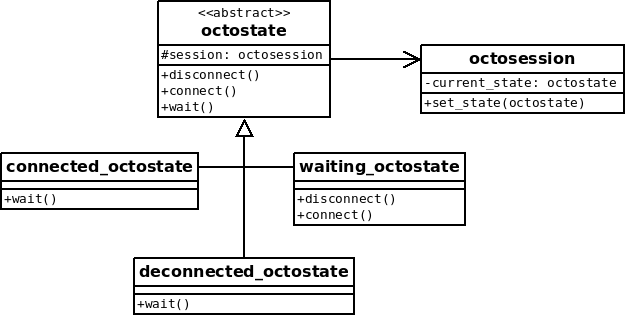
\includegraphics[scale=0.6]{UML/state.png}
				%\input{UML/state.tex}
				\caption{\label{state_uml} Diagramme UML du \textit{pattern state}}
			\end{figure}
			
			\paragraph{}{
			On obtient alors le diagramme à la figure \ref{state_uml}. On a donc trois états, \textit{text}
			}
	\newpage

	\section*{Conclusion}
		\paragraph{}{je conclu}

\end{document}
